\documentclass{article}


\usepackage[utf8]{inputenc}
\usepackage{hyperref}
\usepackage{booktabs}
\usepackage{caption}
\usepackage[flushleft]{threeparttable}
\usepackage{natbib}
\usepackage{graphicx}
\usepackage{subcaption}
\usepackage{listings}
\usepackage[export]{adjustbox}
\usepackage[capitalize]{cleveref}

\usepackage{draftwatermark}
\SetWatermarkText{DRAFT}
\SetWatermarkScale{5}

\newcommand{\findablility}{\textbf{F}indability}
\newcommand{\findable}{\textbf{F}indable}
\newcommand{\accessibility}{\textbf{A}ccessibility}
\newcommand{\accessible}{\textbf{A}ccessible}
\newcommand{\interoperability}{\textbf{I}nteroperability}
\newcommand{\interoperable}{\textbf{I}nteroperable}

\title{FAIR from metadata to the Semantic Web: open source tools and services for data annotation and findable data}

\begin{document}

\maketitle

\begin{abstract}
Annotation of research data with metadata is crucial to provide context for understanding, analysis, re-use, and to overcome the reproducibility crisis. The odML format offers a flexible and comprehensive solution for collecting and organizing metadata in a structured form that is both human readable and machine actionable for documentation and automated analysis. To further support the FAIR principles, we present tools to export metadata from odML to \textit{RDF}\footnote{\url{https://www.w3.org/TR/rdf11-concepts}}, which opens any metadata to \textit{Semantic Web}\footnote{\url{https://www.w3.org/standards/semanticweb}} services. The open source G-Node SPARQL server is aimed at providing searchable whole metadata sets for meta analyses and also providing links to the actual published scientific data set. Scientists can upload their metadata to make their data findable and accessible whether it's published or not.
\end{abstract}

\section{Introduction} \label{sec:introduction}
According to the FAIR principles \cite{Wilkinson_2016}, (meta)data should be \findable{}, \accessible{}, \interoperable{}, and \textbf{R}eusable. Metadata, data about experimental data, play a special role in this context. Not only do they accurately describe the experimental setting and context but ideally also provide information about the data set involved. If handled properly, a collection of metadata is the first step to solving the FAIR principles for a published data set. As previously shown \cite{Teeters_2017} \interoperability{} between even diverse metadata can be achieved by using the common and flexible Semantic Web RDF technology.

Expanding on this idea, we show how \findablility{} and \accessibility{} of large collections of metadata can be achieved by the use of open source software. \interoperability{} between different types of metadata is achieved by a minimal set of common RDF terms. This way diverse sets of metadata can be easily converted and imported into a common searchable data graph. Taking advantage of the powerful OWL feature of RDF, each distinct set of metadata can be sub-classed to the benefit of maintaining the original structure without losing the common generic structure, keeping \interoperability{} without sacrificing \findablility{}.

To make large collections of merged metadata in RDF format easily accessible, we introduce an augmented version of the open source SPARQL server \textit{Apache Fuseki}\footnote{\url{https://jena.apache.org} (Jena 2006, A semantic web framework for Java)}. This software provides access to the metadata by both custom, easy to use search terms as well as the powerful \emph{JG: but harder to master?} %[MS] That SPARQL is hard to master is partially addressed in the usage section and it is mentioned in the outlook that we are aware of it and have a prototype to build a more easy to use query layer on top of SPARQL.
\textit{SPARQL}\footnote{\url{https://www.w3.org/TR/sparql11-query}} query language.

\emph{JG: Do you want to provide a very brief intro to RDF? Similar to what you do for odml?}
%[MS] There is a paragraph introducing RDF in section "sec:why_rdf"; this could be moved here if it makes more sense.

\subsection{The odML data format} \label{sec:odml_intro}
\textit{odML}~\cite{Grewe_2011} is a data format designed to thoroughly document diverse metadata. The odML library~\footnote{\url{https://github.com/G-Node/python-odml} (RRID:SCR\_001376)} is a freely available reference implementation in Python. Developed by the German Neuroinformatics Node (G-Node), its design was oriented along the needs of neuroscientific metadata, but its generic approach makes it applicable to any scientific field and is able to store heterogeneous metadata to fully document even complex experimental setups and conditions \cite{Zehl_2016}.

In brief, the odML concept is to store metadata in a generic but hierarchical structure. Figure ~\ref{fig:odmlModel}A provides an overview of the general odML data model with all its available attributes while Fig ~\ref{fig:odmlModel}B shows an abstraction of how the model can be used to store metadata.

To ease usage, odML features the concepts of terminologies and templates. odML terminologies~\footnote{\url{https://terminologies.g-node.org}} are predefined odML building blocks that can be imported to construct larger but standardized odML documents and further provide the option to give consistent definitions for the defined building blocks. odML templates~\footnote{\url{https://templates.g-node.org}} are fully structured odML documents without actual metadata values meant for re-use in reoccurring experimental settings. Both terminologies and templates can be imported either from local documents or from off-site platforms. The templates~\footnote{\url{https://github.com/G-Node/odml-templates}} and terminologies~\footnote{\url{https://github.com/G-Node/odml-terminologies}} currently published by the G-Node are not meant to be complete and actively encourage community contributions via Github to provide an even larger set of re-useable terminologies and templates available to the general public.

\begin{figure}
   \begin{minipage}[b]{.6\linewidth}
     \centering
     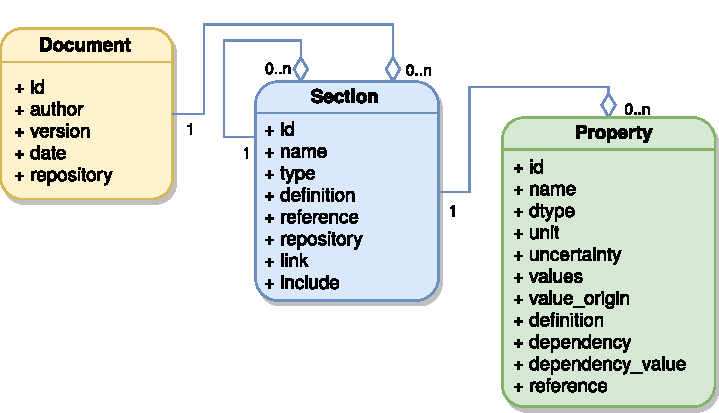
\includegraphics[width=0.9\textwidth]{figures/figOdmlModelA.pdf}
     \subcaption{odML data model}\label{fig:odmlModelData}
   \end{minipage}
   \hfill
   \begin{minipage}[b]{.35\linewidth}
     \centering
     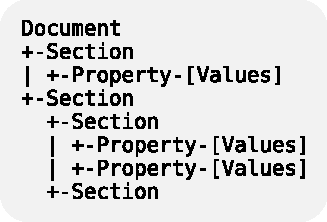
\includegraphics[width=0.9\textwidth]{figures/figOdmlModelB.pdf}
     \subcaption{Abstracted usage example}\label{fig:odmlModelStructure}
   \end{minipage}
   \caption{\textbf{The odML data model.}
(~\ref{fig:odmlModelData}) Entity-relation diagram of the data model. (~\ref{fig:odmlModelStructure}) The two main concept entities are nested \textbf{Sections} that provide a single \textbf{Document} with its general structure and make such a document navigate- and searchable. \textbf{Sections} can contain \textbf{Properties} that in turn contain metadata values.}
   \label{fig:odmlModel}
\end{figure}

\begin{figure}
   \begin{minipage}[b]{.3\linewidth}
     \centering
     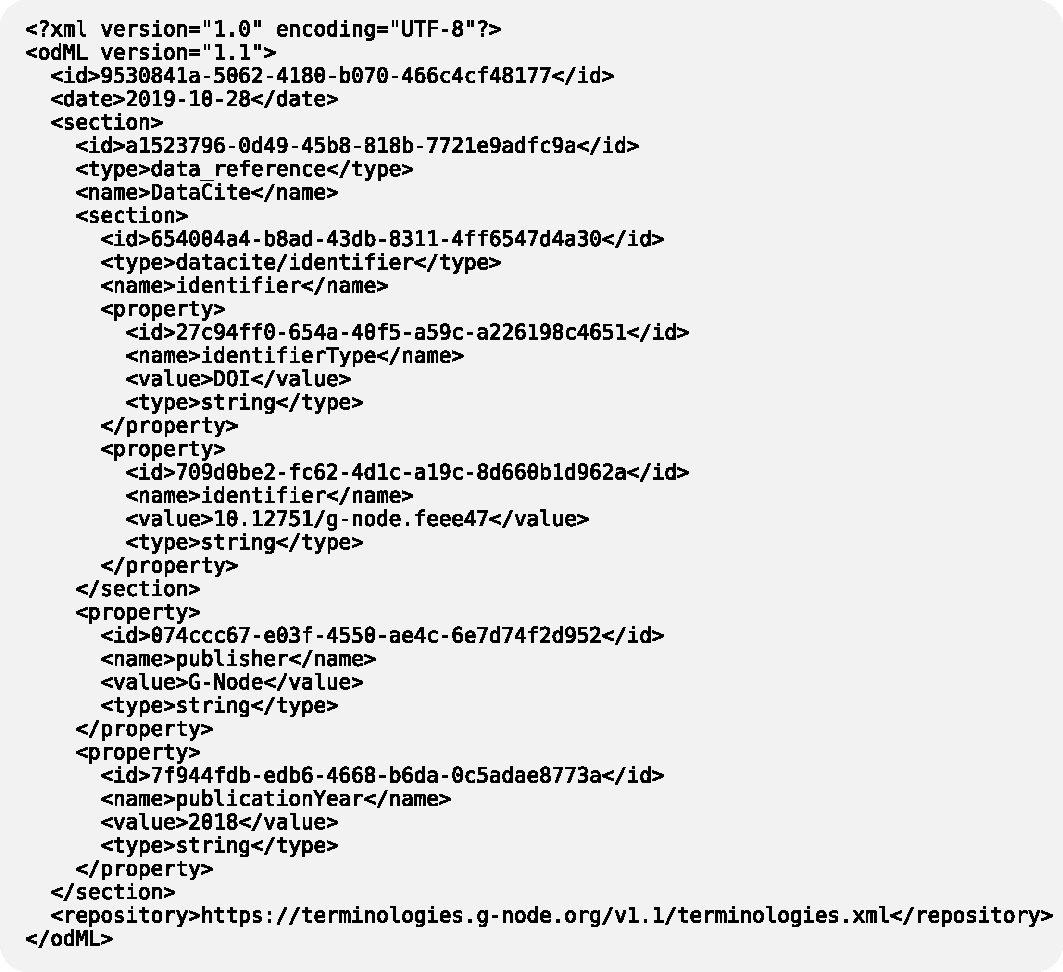
\includegraphics[width=0.99\textwidth]{figures/figFormatExampleA.pdf}
     \subcaption{XML}
     \label{fig:odmlFormatExampleXML}
   \end{minipage}
   \begin{minipage}[b]{.3\linewidth}
     \centering
     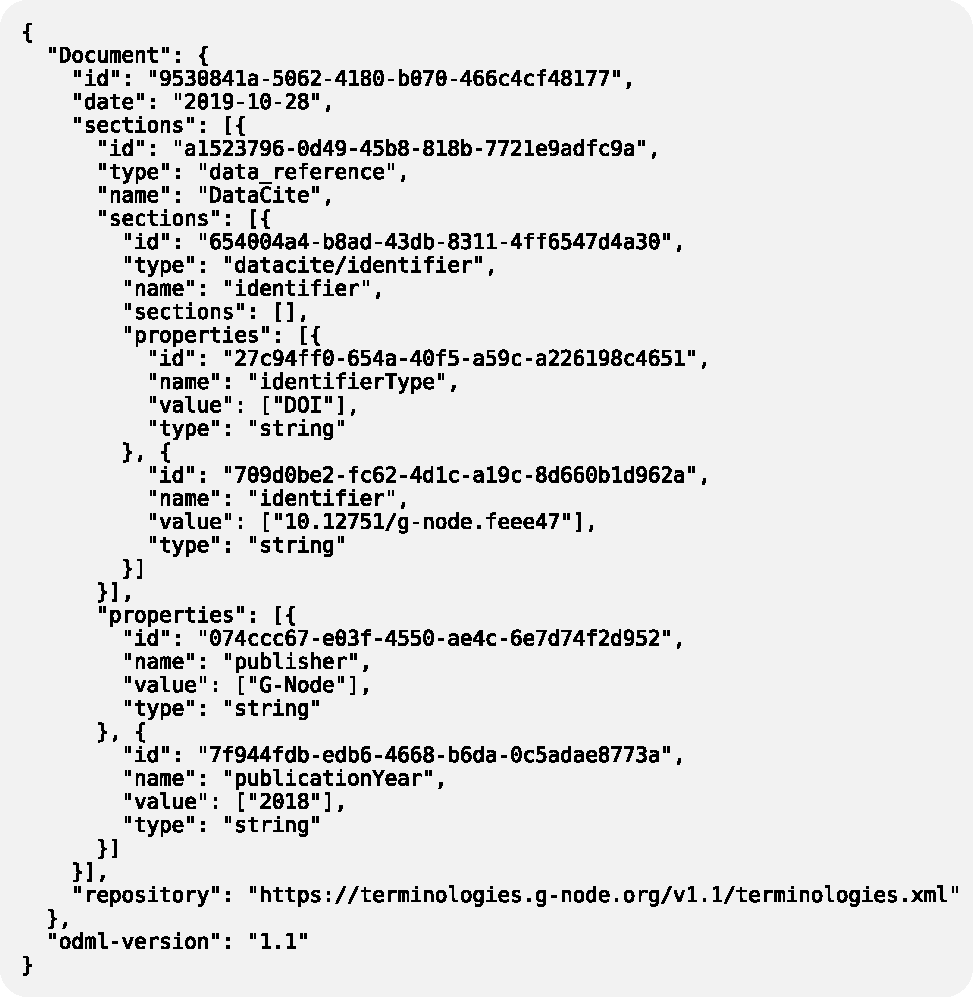
\includegraphics[width=0.99\textwidth]{figures/figFormatExampleB.pdf}
     \subcaption{JSON}
     \label{fig:odmlFormatExampleJSON}
   \end{minipage}
   \begin{minipage}[b]{.3\linewidth}
     \centering
     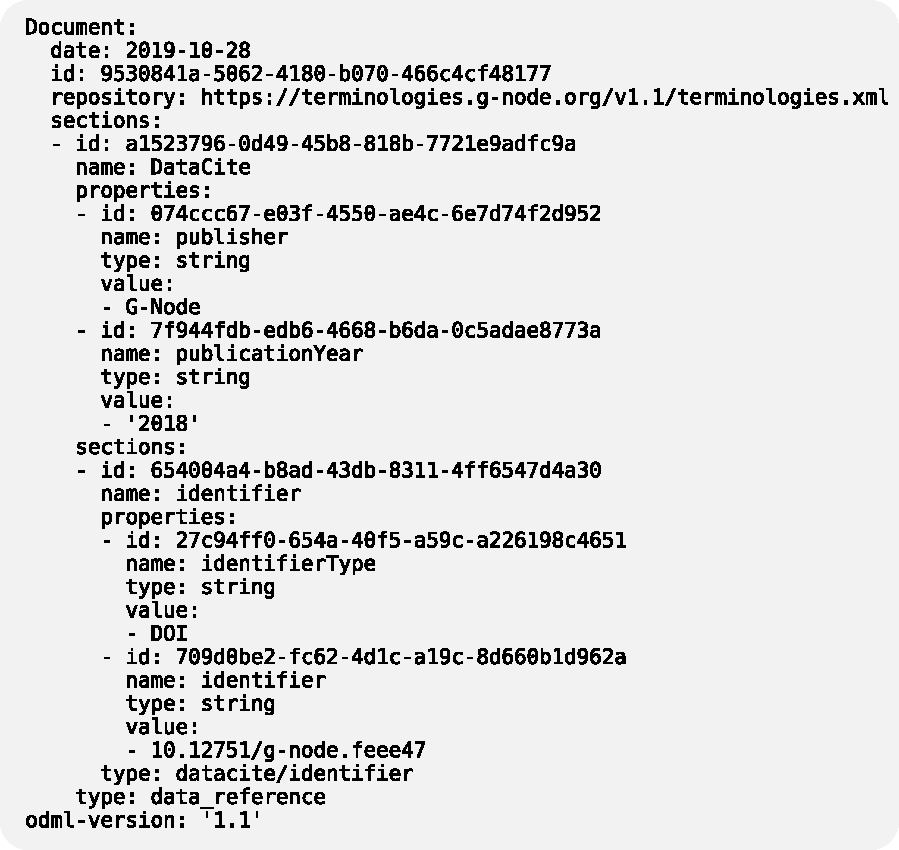
\includegraphics[width=0.99\textwidth]{figures/figFormatExampleC.pdf}
     \subcaption{YAML}
     \label{fig:odmlFormatExampleYAML}
   \end{minipage}
   \caption{Metadata organized in odML and stored using the (~\ref{fig:odmlFormatExampleXML}) XML, (~\ref{fig:odmlFormatExampleJSON}) JSON and (~\ref{fig:odmlFormatExampleYAML}) YAML storage formats. While both XML and JSON are well used in data processing and automation, YAML provides an option for both human readability and machine consumption.}
   \label{fig:odmlFormatExample}
\end{figure}

Metadata organized using the odML data model can be stored in different file formats: XML, JSON and YAML. See Fig~\ref{fig:odmlFormatExample} for examples. The figures show parts of the DataCite\footnote{\url{https://datacite.org}} schema as an example since it will serve later on as one of the main search criteria to find and link back to published or otherwise available datasets. We provide a full DataCite odML terminology
%[TW] odML terminologies should be introduced %[MS] added a paragraph before the file format description paragraph above to not break the reading flow at this point. Can be changed if it works better at another location.
\footnote{\url{https://terminologies.g-node.org/v1.1/datareference/datacite.xml}}, two specific odML templates \footnote{\url{https://templates.g-node.org/datacite/datacite.crcns.xml}}\footnote{\url{https://templates.g-node.org/datacite/datacite.gnode.xml}} as a reference usage implementation and a Python conversion script from XML Datacite files to odML \footnote{\url{https://github.com/G-Node/odmltools}}.


\subsection{Opening odML to graph database searches} \label{sec:why_rdf}

While odML has shown to document experiments even through diverse fields due to its flexibility, there is a growing need to search metadata across multiple experiments as well as across multiple fields. As recently published \cite{Sprenger_2019}, the odML data format has been developed further to also address this growing demand.

Even though searches within extensive odML documents were always part of the implementation and imports from linked, external sources into individual documents are possible, the option to easily search across multiple documents was still lacking. To this end we chose to open the odML data format to the \textit{Semantic Web}\footnote{\url{https://www.w3.org/standards/semanticweb}} via conversion to the \textit{RDF (Resource Description Framework)}\footnote{\url{https://www.w3.org/TR/rdf11-concepts}} format.

RDF was designed by the World Wide Web Consortium (W3C)\footnote{\url{https://www.w3.org}} as a standard model for data representation and exchange on the web with the heterogeneity of data in mind. Even though the RDF file format might vary, the underlying concept features two key points. The first is that information is structured in subject-predicate-object triples e.g. \texttt{apple hasColor red}. The second key point is that multiple subjects and objects can be connected to form a graph e.g. \texttt{tree hasFruit apple} can be combined with the previous example to form a minimal graph. These graphs can contain very heterogeneous data, but can still be queried due to the semantic structure of the underlying data\footnote{\url{https://www.w3.org/TR/rdf11-concepts}}.

The Semantic Web offers a large, freely available technology stack fit to adopt, query and publish custom metadata graphs: A suite of various graph database tools to merge individual documents in the RDF format into a single graph even if the content of the documents are not uniform. SPARQL (SPARQL Protocol and RDF Query Language), a full fledged query language that can be used to extract information from such a graph. Another feature is \textit{OWL (Web Ontology Language)}\footnote{\url{https://www.w3.org/TR/owl-ref}} which enables the definition of a vocabulary extension of the basic RDF terminology to enable more elaborate and domain specific SPARQL searches. The broad range of freely available open source tools can be adapted to fit more specific use cases.

\section{Implementation} \label{sec:implementation}

This section describes how the versatile odML data format was mapped to its RDF equivalent and documents the specific OWL ontology that was devised for the underlying data model. It also shows how metadata can be exported from odML to its RDF equivalent, how different documents can be loaded into a single graph and how the graph can be searched via SPARQL. It will be shown how the basic structure can be furthered with individual sub-classes to make searches more specific. Finally it will present an open web service that enables metadata searches across multiple documents and present a suggestion based on the widely accepted \textit{DataCite}\footnote{\url{https://datacite.org}} publication standard to enable back-links from metadata sets to the original, published data.

\subsection{Implementation of odML to RDF mapping} \label{sec:odml_rdf}

%[TW] address the implications of the odML hierarchical structure for the mapping between odml and rdf
%[MS] not sure if I fully got the comment, but I went a bit more into detail with respect to the mapping in the following paragraph
%[TW] You should describe the data model structures of RDF and odML to make it clear that a mapping is not trivial. When you describe the mapping you should address these differences and how they are accounted for.

odML is by design a hierarchical data format meant to accommodate heterogeneous data. This provides a common, underlying structure which enables people unfamiliar with the details of a documented experiment to navigate such a document. The same is true when odML is mapped to RDF. Since RDF is meant to enable searches over graph databases with heterogeneous data, a graph containing odML specific data already shows a common, underlying structure making useful searches easier even across unfamiliar sets of data.

The initial step in the odML to RDF export was to map the odML entities \texttt{Document}, \texttt{Section} and \texttt{Property} to RDF classes and provide the respective RDF predicates and XSD\footnote{\url{https://www.w3.org/TR/xmlschema11-2}} types.

\subsubsection{Mapping of odML entities to RDF classes} \label{sec:odml_rdf_mapping}

A common concept in computing is the namespace, which is used to uniquely identify an entity that might occur in a different context within the same dataset. In this context the namespace usually consists of a global identifier and a local name that might otherwise be ambiguous, e.g., in the Python import statement \texttt{http.server}, \texttt{http} is the global identifier while \texttt{server} is the local name.
In the Semantic Web the global identifier is called \texttt{namespace IRI}\footnote{\url{https://www.w3.org/TR/rdf-syntax-grammar\#section-Namespace}} (Internationalised Resource Identifier) and is used to distinguish entities from different Datasets. The IRI of RDF for example is \texttt{http://www.w3.org/1999/02/22-rdf-syntax-ns\#}. For odML RDF, the namespace \url{https://g-node.org/odml-rdf} was chosen to identify all RDF odML entities.

For the actual mapping, the odML entities \texttt{Document}, \texttt{Section} and \texttt{Property} where mapped to RDF Classes, while all attributes of the individual odML entities, e.g. \texttt{id} or \texttt{reference} where mapped to RDF Literals. An exception is the \texttt{Property.values} that requires a container element, the \texttt{RDF.Seq}. This was necessary since an RDF graph does not retain any order between its contained triples. \texttt{RDF.Seq} is a class that allows to specify an order of the contained elements. Only this allows an exact export of odML values to RDF, where the order of values often is actually important, for example in the case of documenting a set of stimuli. \cref{table:Document,table:Section,table:Property,table:Hub,table:Terminology} describe the mapping in detail.

\begin{table}
\begin{threeparttable}
\begin{tabular}{p{3.5cm}p{5cm}p{2cm}}
\toprule
    odml                    & RDF                                 & xsd type \\
\midrule
    odml (a)                & odml:Document                       & - \\
                            & & \\
    id (b)                  & RDF node instance name              & - \\
    author                  & odml:hasAuthor                      & xsd:string \\
    date                    & odml:hasDate                        & xsd:date \\
    version (odml)          & odml:hasVersion                     & xsd:float \\
    version (document)      & odml:hasDocVersion                  & xsd:string \\
    repository (c)          & odml:hasTerminology                 & - \\
                            & odml:hasExternalTerminology         & xsd:string \\
    Sections                & odml:hasSection                     & - \\
    - (d)                   & odml:hasFilename                    & xsd:string \\
\bottomrule
\end{tabular}
\caption{odML Document}
\begin{tablenotes}
\small
\item Mapping of odML \texttt{Document} to RDF. (a) The document root is mapped to an RDFS class of type \texttt{odml:Document}. (b) The UUID of the odML \texttt{Document} is used as Name of the created \texttt{odml:Document} RDF node to uniquely identify the document if it is merged with a graph database. (c) RDF export of repositories: linked terminologies are downloaded on conversion and exported additional RDF document connected via the \texttt{odml:Hub} RDF node. This additional document is linked via \texttt{odml:hasTerminology} to the original document. If the terminology cannot be imported, its URL will be kept as is and its value is provided as an RDF leaf via the predicate \texttt{odml:hasExternalTerminology} in the original document. See ~\ref{table:Hub} and ~\ref{table:Terminology} for more detailed descriptions.
(d) As provenance from where the RDF odml:Document was created from, the filename of the original odML file is documented via the non-odML format predicate \texttt{odml:hasFilename}.
\end{tablenotes}
\label{table:Document}
\end{threeparttable}
\end{table}

\begin{table}
\begin{threeparttable}
\begin{tabular}{p{3.5cm}p{5cm}p{2cm}}
\toprule
    odml            & RDF                             & xsd type \\
\midrule
    Section (a)     & odml:Section                    & - \\
                    & & \\
    id (b)          & RDF node instance name          & - \\
    name            & odml:hasName                    & xsd:string \\
    type            & odml:hasType                    & xsd:string \\
    definition      & odml:hasDescription             & xsd:string \\
    repository (c)  & odml:hasTerminology             & - \\
                    & odml:hasExternalTerminology     & xsd:string \\
    reference (d)   & odml:hasReference               & xsd:string \\
    Sections (e)    & odml:hasSection                 & - \\
    Properties      & odml:hasProperty                & - \\
\bottomrule
\end{tabular}
\caption{odML Section}
\begin{tablenotes}
\item Mapping of odML \texttt{Section} to RDF. (a) Any odML \texttt{Section} entity is mapped to an RDFS class of type \texttt{odml:Section}. (b) The UUID of an odML \texttt{Section} entity is used as Name of the created \texttt{odml:Section} RDF node to uniquely identify the section if it is merged with a graph database. If this node already exists in the graph, it will not add a duplicate entry, but will add only any predicates that the graph with respect to this Section node does not already contain.
(c) cf. \texttt{repository} description in Table ~\ref{table:Document}. (d) A \texttt{reference} can either be a URL to an external reference or a string pointing to an id in a Database. (e) Unspecific Sections are exported using the \texttt{odml:Section} class and the \texttt{odml:hasSection} predicate. We also provide a set of "specialized" RDF classes that are sub-classes of Section. cf. ~\ref{sec:rdf_subclassing} for details.
\end{tablenotes}
\label{table:Section}
\end{threeparttable}
\end{table}

\begin{table}
\begin{threeparttable}
\begin{tabular}{p{3.5cm}p{5cm}p{2cm}}
\toprule
    odml            & RDF                           & xsd type \\
\midrule
    Property (a)    & odml:Property                 & - \\
                    & & \\
    id (b)          & RDF node instance name        & - \\
    name            & odml:hasName                  & xsd:string \\
    definition      & odml:hasDefinition            & xsd:string \\
    reference (c)   & odml:hasReference             & xsd:string \\
    unit            & odml:hasUnit                  & xsd:string \\
    dtype           & odml:hasDtype                 & xsd:string \\
    uncertainty     & odml:hasUncertainty           & xsd:float \\
    values (d)      & odml:hasValue                 & - \\
                    & rdf:Seq                       & - \\
                    & rdf:\_\#                      & xsd:string \\
    value\_origin    & odml:hasValueOrigin           & xsd:string \\
\bottomrule
\end{tabular}
\caption{odML Property}
\begin{tablenotes}
\item mapping of odML \texttt{Property} to RDF. (a) Any odML \texttt{Property} entity is mapped to an RDFS class of type \texttt{odml:Property}. (b) The UUID of an odML \texttt{Property} entity is used as Name of the created \texttt{odml:Property} RDF node to uniquely identify the section if it is merged with a graph database. (c) cf. \texttt{reference} description in Table ~\ref{table:Section}. (d) odML supports multiple values. Upon export to RDF the order of these values need to be respected as well. Values are connected to the RDF document via the \texttt{odml:hasValue} predicate to an \texttt{rdf:Seq} node. This \texttt{rdf:Seq} node in turn contains numbered \texttt{rdf:li} items which in turn contain the individual \texttt{odml.Value entries}. This construct enables RDF searches for individual values rather then searching for lists of values.
\end{tablenotes}
\label{table:Property}
\end{threeparttable}
\end{table}

\begin{table}
\begin{threeparttable}
\begin{tabular}{p{3.5cm}p{5cm}p{2cm}}
\toprule
    odml            & RDF                           & xsd type \\
\midrule
    -               & odml:Hub                      & - \\
    -               & odml:hasDocument              & - \\
    -               & odml:hasTerminology           & - \\
\bottomrule
\end{tabular}
\caption{Hub}
\begin{tablenotes}
\item The custom RDF type of class \texttt{odml:Hub} has no odML entity equivalent. It is introduced to merge Documents and Terminologies into a single RDF graph: the "Hub" is used to root a graph that might contain multiple documents to enable searches across unrelated and in-homogeneous metadata content.
\end{tablenotes}
\label{table:Hub}
\end{threeparttable}
\end{table}

\begin{table}
\begin{threeparttable}
\begin{tabular}{p{3.5cm}p{5cm}p{2cm}}
\toprule
    odml            & RDF                               & xsd type \\
\midrule
    -               & odml:Terminology                  & - \\
    Sections        & odml:hasSection                   & - \\
\bottomrule
\end{tabular}
\caption{Terminology}
\begin{tablenotes}
\item odML documents can link to external Terminology documents. To make these available for searches within a connected RDF graph besides the odML documents they are referenced by, linked terminologies are imported and converted into RDF documents. They are connected via the \texttt{odml:hasSection} predicate to their referencing documents. Conversely the \texttt{odml:Section} in an \texttt{odml:Document} references the Terminology via the \texttt{odml:hasTerminology} predicate.
\end{tablenotes}
\label{table:Terminology}
\end{threeparttable}
\end{table}

\begin{figure}
\begin{center}
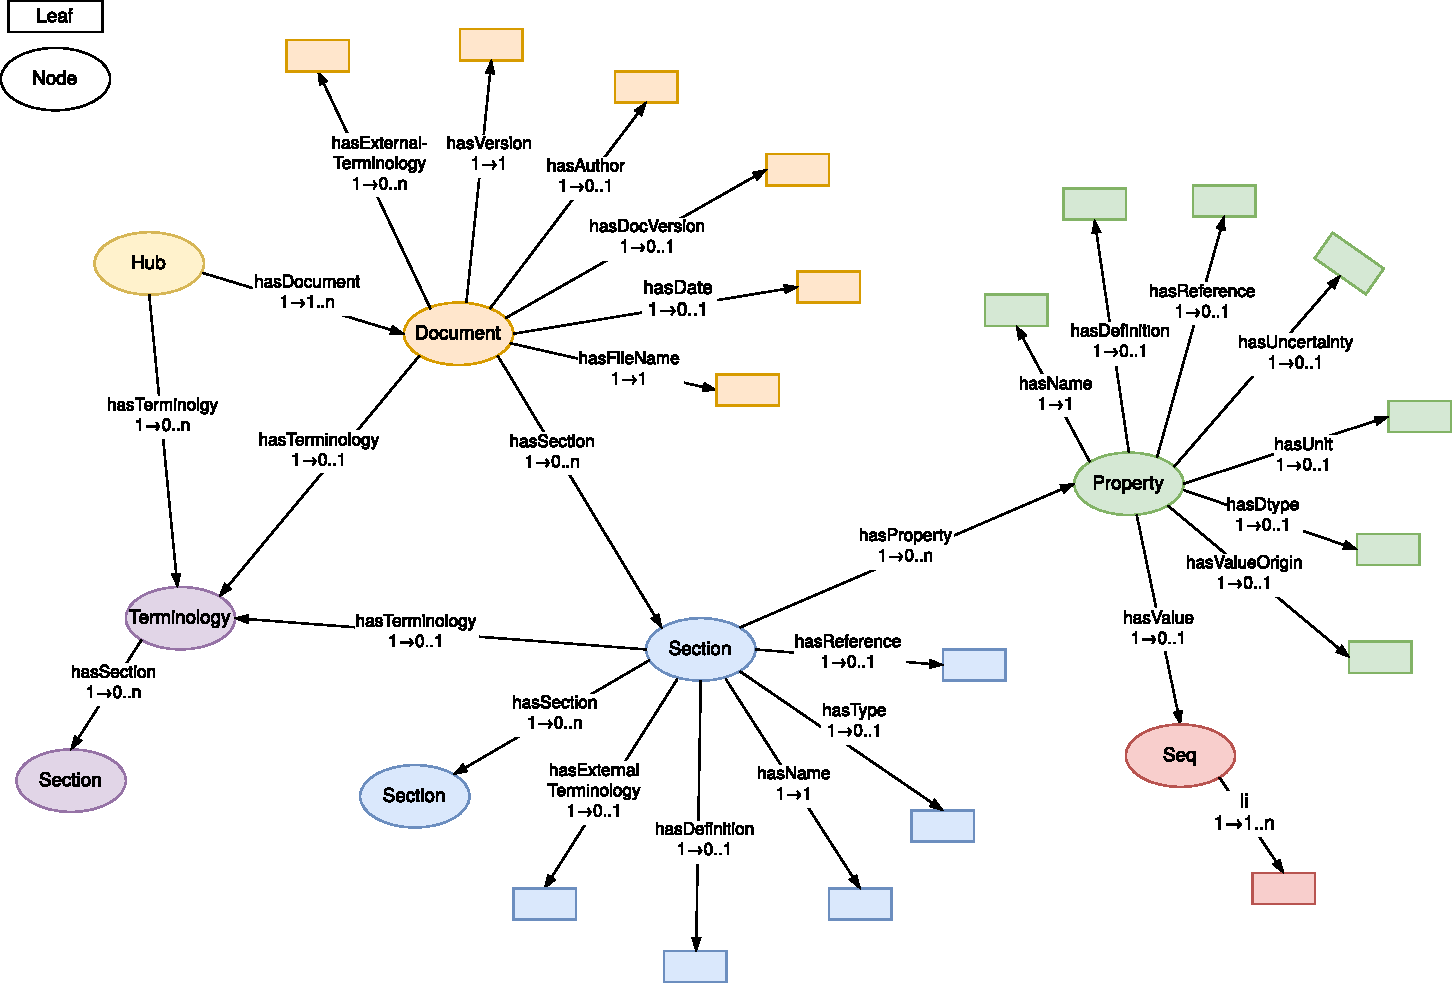
\includegraphics[width=0.90\columnwidth]{figures/odmlRDFDataModel.pdf}
\caption{The odML RDF data model.}
\label{fig:rdfModel}
\end{center}
\end{figure}

\subsubsection{Subclassing of Sections} \label{sec:rdf_subclassing}
All of the RDF Classes can be fine grained into Subclasses to give more semantic meaning to the connection between nodes. For example \texttt{section hasSection section} becomes \texttt{section hasExperimenter section}. Here \texttt{hasExperimenter} is a subclass of \texttt{hasSection}. A search for a class will return as a result all its subclasses as well. Using our current example, a search for \texttt{hasExperimenter} returns only sections connected via this specific property, while a search for \texttt{hasSection} returns all sections connected by \texttt{hasSection} as well as \texttt{hasExperimenter}.

\subsubsection{odML RDF ontology} \label{sec:odml_ontology}
To make use of the RDF feature of validating individual RDF files, we created an odML RDF ontology which includes the basic set of odML RDF terms and included all currently supported Section sub-classes. The complete file can be found in the Appendix under Listing ~\ref{lst:ontology}. This list of sub-classes should not be seen as permanent and is expected to increase in the future.

\subsection{Creating odML and converting to RDF} \label{sec:odml_to_rdf}

\subsubsection{Converting odML to RDF} \label{sec:odml_conversion}
The default odML Python library\footnote{\url{https://github.com/G-Node/python-odml} (RRID:SCR\_001376)} installation automatically provides a convenience command line script that converts odML files to their RDF pendant.

\begin{lstlisting}[label=lst:conversion_script, caption=odML to RDF conversion Python script]
$ odmltordf [-r] [-o OUT] SEARCHDIR
\end{lstlisting}

\texttt{SEARCHDIR} All odML files in the specified directory will be converted to RDF.
\texttt{-r} An optional argument to include directories recursively.
\texttt{-o OUT} An optional argument to specify an output directory.

\subsubsection{Using the DataCite schema to annotate published datasets} \label{sec:datacite}
As stated above, we encourage using the DataCite schema\footnote{\url{https://datacite.org}} to provide the basic description of a published dataset since it is an adopted and widely accepted standard in the annotation of datasets. We provide a dedicated, fully compatible terminology for the DataCite standard in odML\footnote{\url{https://terminologies.g-node.org/v1.1/datareference/datacite.xml}}. We also provide a convenience script to convert an existing DataCite XML file into an odML file\footnote{\url{https://github.com/G-Node/odmltools}}. Once installed, the odML package provides a command line script that can be used to convert DataCite XML files to odML:

\begin{lstlisting}[label=lst:datacite_script, caption=Datacite import Python script]
$ odmlimportdatacite [-f FORMAT] [-o OUT] [-r] [-p] INPUT
\end{lstlisting}

\texttt{INPUT} Path and filename of the DataCite XML file to be parsed. If used with the [-r] flag, INPUT should be a directory; all DataCite XML files within this directory and any sub directories will be parsed to odML.
\texttt{-F FORMAT} odML output file format. Available formats are 'XML', 'JSON', 'YAML', 'RDF'. Default format is 'XML'.
\texttt{-o OUT} Output directory. Must exist if specified. If not specified, output files will be written to the current directory.
\texttt{-r} An optional argument to walk recursively through a repository and convert all DataCite files found.
\texttt{-p} An optional argument to print the parsed document tree(s) to the command line.

The script can be used to directly convert a DataCite XML file to RDF

An existing odML file which was used to document a published set of experiments can easily be combined with an odML file created from a DataCite XML file and saved to RDF.

\subsection{Working with an odML RDF graph} \label{sec:rdf_usage}

There are various different libraries that allow creating local graph databases and querying the contents. Two prominent examples are the Java Apache Jena Suite\footnote{\url{https://jena.apache.org}} and the Python rdflib\footnote{\url{https://rdflib.readthedocs.io/en/stable}} library package. In the following paragraphs the code examples will be using Python with the rdflib package to demonstrate how to work with an odML RDF graph.

\subsubsection{Creating an odML RDF graph} \label{sec:rdf_graph_create}

Code listing ~\ref{lst:create_graph} shows how to create an in-memory RDF graph from two example odML RDF files. The content of the example files can be found in the appendix.

\begin{lstlisting}[label=lst:create_graph, caption=Create RDF graph, basicstyle=\small]
from rdflib import Graph

# Path to two example odML RDF files that will be loaded
# and merged into a single graph.
odml_file_A = './example_A_odml.rdf'
odml_file_B = './example_B_odml.rdf'

# Create a new empty graph
local_graph = Graph()

# Load the contents of both files into a single graph
local_graph.parse(odml_file_A)
local_graph.parse(odml_file_B)
\end{lstlisting}

\subsubsection{How to query an odML RDF graph} \label{sec:rdf_graph_query}
The following SPARQL query example shows how a graph containing multiple DataCite odML documents can be queried for DataCite "Subjects" (Keywords) and retrieve the DOI identifier linking back to these corresponding data sets.

The following query uses the graph created in the previous example.

\begin{lstlisting}[label=lst:query_graph, caption=Example query, basicstyle=\small]
from rdflib import RDF, RDFS, Namespace
from rdflib.plugins.sparql import prepareQuery

# Providing the namespaces that will be used in the query
ns_dict = {"odml": Namespace("https://g-node.org/odml-rdf#"),
           "rdf":RDF}

# Preparing the query string
query = """SELECT DISTINCT *
WHERE {
  ?doc rdf:type odml:Document .
  ?doc odml:hasFileName ?file .
  ?doc odml:hasSection* ?sec_id .
  ?sec_id odml:hasProperty ?prp_id .
  ?prp_id odml:hasName "identifier" .
  ?prp_id odml:hasValue ?val_doi .
  ?val_doi ?pred_doi ?doival .

  ?doc odml:hasSection* ?sec_subj .
  ?sec_subj odml:hasType "datacite/subject" .
  ?sec_subj odml:hasProperty ?prp_subj .
  ?prp_subj odml:hasValue ?val_subj .
  ?val_subj ?pred_subj ?keyword .
  {?val_subj ?pred_subj "Neuroscience"} UNION
  {?val_subj ?pred_subj "Electrophysiology"} .

  FILTER regex(str(?pred_doi), '_')
  BIND(CONCAT("https://doi.org/", STR(?doival)) as ?doi_link)
}"""
prep_query = prepareQuery(query, initNs=ns_dict)

# Printing the results
for row in local_graph.query(prep_query):
    print("""
    File: %s
    DOI: %s
    Keyword: %s\n""" % (row.file, row.doi_link, row.keyword))
\end{lstlisting}

This query will return DOI links to the data sets with Keywords "Neuroscience" and "Electrophysiology". As additional information it also provides the filename of the original metadata file, the type of Identifier, and the matching keyword. Likewise a search could start from searching for specific authors of a data set. The results of the query in ~\ref{lst:query_graph} can be found in ~\ref{lst:query_result}.

\begin{lstlisting}[label=lst:query_result, caption=Query result, basicstyle=\small]
    File: example_A_odml.xml
    DOI: https://doi.org/10.12751/g-node.no_doi_A
    Keyword: Electrophysiology

    File: example_B_odml.xml
    DOI: https://doi.org/10.12751/g-node.no_doi_B
    Keyword: Neuroscience
\end{lstlisting}

\subsubsection{How to use subclassing to reduce query overhead} \label{sec:rdf_subclass_usage}

As seen in the example above, queries with the basic odML structure can become quite extensive. Even tough SPARQL provides powerful tools for subqueries and filtering of results we were aiming at making such queries more intuitive. To this end you can find a list of Section subclasses in the odML OWL ontology\footnote{\url{https://g-node.org/odml-rdf}}. Subclasses can be queried directly without needing to know the odML type of a class. In the example one can directly query for \texttt{odml:Subject} and does not need to know that the corresponding Section is of type \texttt{datacite/subject}.

The following query requires the imports and uses the graph created in the previous example.

\begin{lstlisting}[label=lst:query_graph_subclass, caption=Subclass query example, basicstyle=\small]
query = """
SELECT DISTINCT * WHERE {
  ?doc a odml:Document .
  ?doc odml:hasFileName ?file .

  ?doc odml:hasSection* ?sec_id .
  ?sec_id odml:hasProperty ?prp_id .
  ?prp_id odml:hasName "identifier" .
  ?prp_id odml:hasValue ?prp_doi_val .
  ?prp_doi_val ?pred_doi ?doival .

  ?doc odml:hasSection* ?sec_subj .
  ?sec_subj a odml:Subject .
  ?sec_subj odml:hasProperty ?prp_subj .
  ?prp_subj odml:hasValue ?val_subj .
  ?val_subj ?pred_subj ?keyword .
  {?val_subj ?pred_subj "Neuroscience"} UNION
  {?val_subj ?pred_subj "Electrophysiology"} .

  FILTER regex(str(?pred_doi), '_')
  BIND(CONCAT("https://doi.org/", STR(?doival)) as ?doi_link)
}
"""
prep_query = prepareQuery(query, initNs=ns_dict)
for row in local_graph.query(prep_query):
    print("""
    File: %s
    DOI: %s
    Keyword: %s\n""" % (row.file, row.doi_link, row.keyword))
\end{lstlisting}

This query will lead to the same result as the original query in code listing ~\ref{lst:query_graph}.

\subsection{Implementation of a SPARQL server: meta.g-node.org} \label{sec:odml_query}

Fuseki is an open source SPARQL query server from the \textit{Apache Jena}\footnote{\url{https://jena.apache.org} (Jena 2006, A semantic web framework for Java)} Semantic Web tools suite that was adopted to support odML specific RDF. A publicly accessible instance is available at https://meta.g-node.org. The service provides a metadata graph searchable by SPARQL containing all scientific Datasets that have been published by \textit{CRCNS (Collaborative Research in Computational Neuroscience)}\footnote{\url{https://crcns.org}} and \textit{G-Node}\footnote{\url{https://doid.gin.g-node.org}}. The server provides example SPARQL queries how the available database can be used. The service is free to use and free to contribute, any additions to the database are welcome and encouraged.

The SPARQL server including all example queries has been dockerized. Both source code\footnote{\url{https://github.com/G-node/odml-query}} and docker container\footnote{\url{https://hub.docker.com/r/gnode/meta}} are freely available and free to use. The repository contains information how to set up an in-house instance and upload odML rdf files to a common graph.

The following is the same query as the one shown above in the local query. The SPARQL queries work slightly differently in the Java Apache Jena and the Python rdflib implementation.

\begin{lstlisting}[label=lst:query_server, caption=Example query server, basicstyle=\small]
prefix rdf: <http://www.w3.org/1999/02/22-rdf-syntax-ns#>
prefix odml: <https://g-node.org/projects/odml-rdf#>

SELECT SAMPLE(?keyword) ?file ?doi_link
WHERE {
  ?doc rdf:type odml:Document .
  ?doc odml:hasFileName ?file .
  ?doc odml:hasSection* ?sec_id .
  ?sec_id odml:hasProperty ?prp_id .
  ?prp_id odml:hasName "identifier" .
  ?prp_id odml:hasValue ?val_doi .
  ?val_doi ?pred_doi ?doival .

  ?doc odml:hasSection* ?sec_subj .
  ?sec_subj odml:hasType "datacite/subject" .
  ?sec_subj odml:hasProperty ?prp_subj .
  ?prp_subj odml:hasValue ?val_subj .
  ?val_subj ?pred_subj ?keyword .
  {?val_subj ?pred_subj "Neuroscience"} UNION
  {?val_subj ?pred_subj "Electrophysiology"} .

  FILTER regex(str(?pred_doi), '_')
  BIND(CONCAT("https://doi.org/", STR(?doival)) as ?doi_link)
}
GROUP BY ?file ?doi_link
ORDER BY ?file
LIMIT 50
\end{lstlisting}


\subsection{Suggested workflow} \label{sec:odml_rdf_workflow}

The suggested workflow can be seen in Figure ~\ref{fig:workflowSchema}

\begin{figure}
\begin{center}
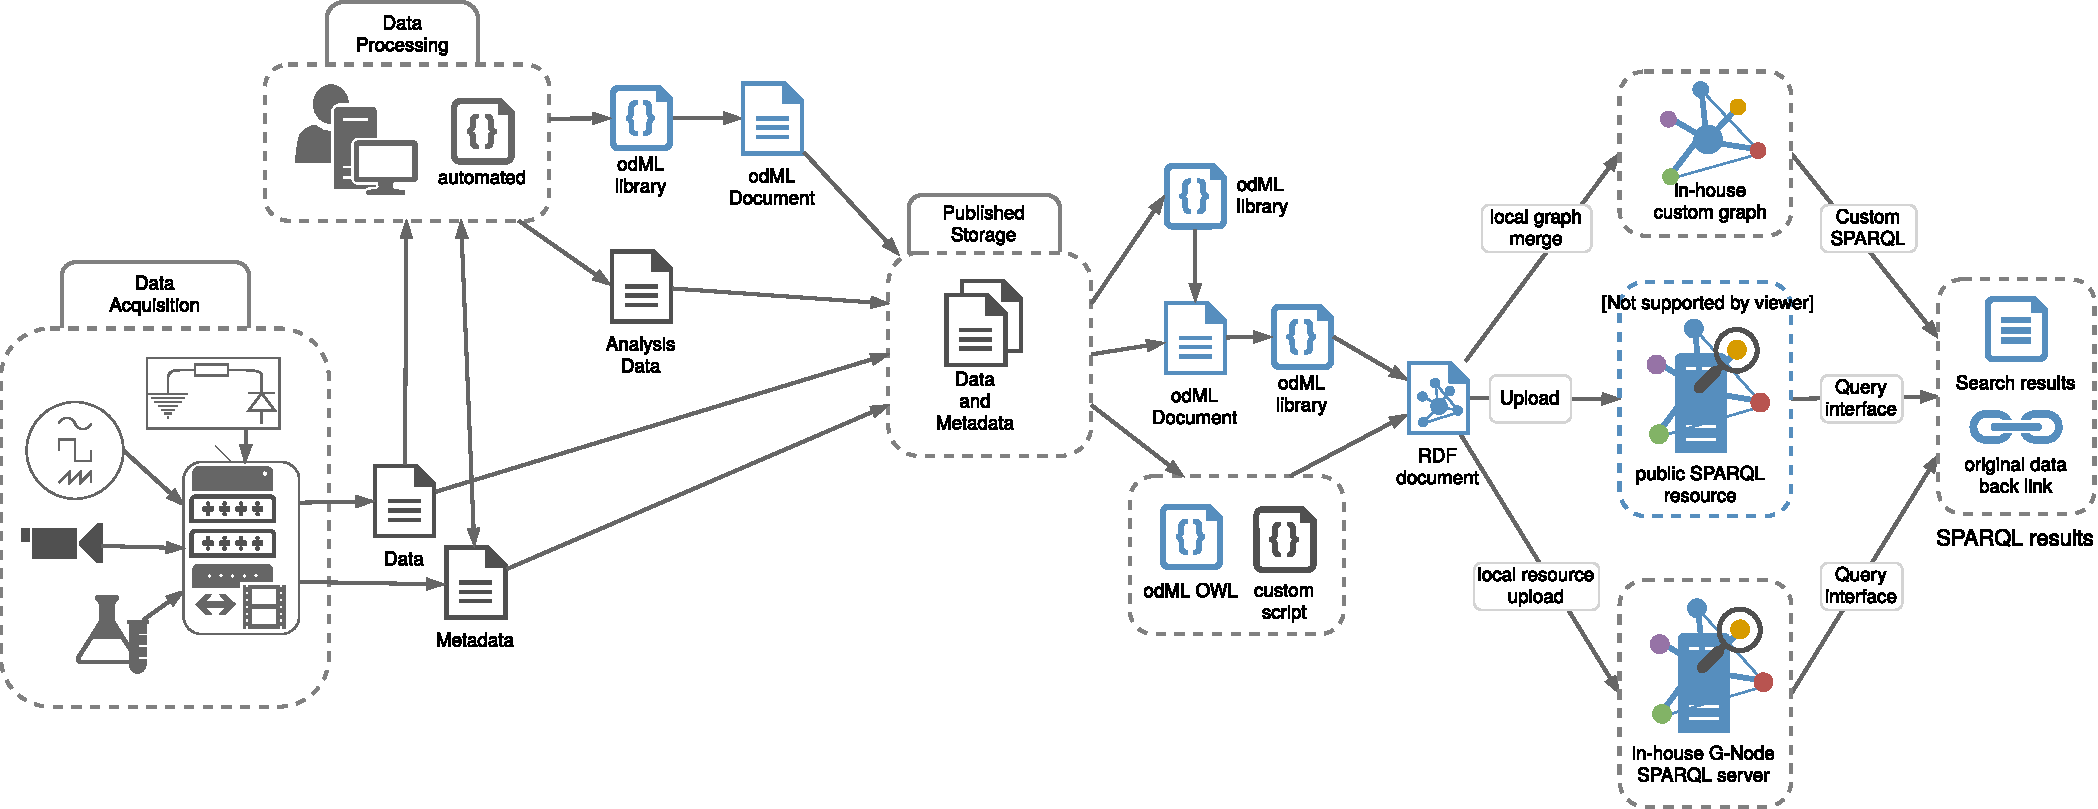
\includegraphics[width=0.90\columnwidth]{figures/workflowSchema.pdf}
\caption{The figure describes possible metadata workflows from an experiment to a graph database.}
\label{fig:workflowSchema}
\end{center}
\end{figure}

\section{(Sort of) Discussion}

\subsection{The flexibility of an odML RDF graph and complexity of queries}

One might argue that a relational database would be better suited to metadata storage and indexing. This argument has merit, since a dedicated database with a predetermined schema (i.e., fixed tables and named columns) can provide more specific queries.
A main problem that arises at this point is the diversity of metadata that is used to describe scientific experiments. If various experiments are described in detail, the resulting metadata will most likely be heterogeneous. odML aims at providing a general, common data structure while providing the required flexibility to accommodate all of these heterogeneous metadata. The conversion to RDF is a logical extension of this approach: with converting odML data to RDF and merging the resulting documents into a single graph, heterogeneous metadata are combined into a single database. This database can be queried due to the underlying hierarchical odML structure when a comparable relational database could not accommodate the necessary different tables for every individual way experiments were described.
The necessary complex SPARQL queries are both an advantage and a disadvantage: Searching across such a complex graph will often necessitate multiple steps to arrive at the required result. A user first has to search for specifics, e.g., data sets that contain keywords, authors, specific hardware or is describing stimuli or was using specific scientific models. All of this can be documented and queried via odML RDF but will require a set of query steps to arrive from the initial search results at a result with links back to the original data sets.
We are aware of this issue. A first step to simplify searches has already been done and described by providing a subclassing system to reduce the query complexity while keeping the underlying basic data model intact. A step further could be the introduction of an abstraction layer that automatically converts a simple keyword based search into useful SPARQL queries. The current python odML library contains a prototype of such an abstraction and is briefly described in the outlook section.

\section{Outlook} \label{sec:outlook}
\subsection{Multiple Endpoint queries} \label{sec:outlook_endpoints}
SPARQL is able to query multiple graphs that are not necessarily part of the same resource. In theory multiple labs can run their own odML SPARQL servers and all that is required to use such resources combined are the URLs where the graphs are available as SPARQL endpoints. A SPARQL query can then be devised which can run over multiple known metadata graphs end return a single result set from various sources.

As an abstracted example, a query across two graphs would be constructed like the following code; a complete example requires an IRI to an available SPARQL endpoint.

\begin{lstlisting}[label=lst:multi_graph, caption=Abstract multiple graph query, basicstyle=\small]
SELECT ?sec_name WHERE {
  {
  GRAPH <https://CUSTOM_ODML_RDF_SOURCE_IRI> {
    ?section ?odml:hasType "datacite" .
    ?section ?odml:hasName ?sec_name }
  }
  UNION
  {
  GRAPH <https:/meta.g-node.org> {
    ?section ?odml:hasType "datacite" .
    ?section ?odml:hasName ?sec_name }
  }
}
\end{lstlisting}

\subsection{Custom subclassing}\label{sec:outlook_subclassing}
As discussed above and can be found in the odML OWL ontology\footnote{\url{https://github.com/G-Node/python-odml/blob/master/odml/resources/odml-ontology.ttl}}, odML RDF features a set of specific Subclasses to reduce the complexity of SPARQL queries. The current implementation of odML RDF provides a mechanism to provide and use a custom list of Subclasses when converting odML to RDF. All definitions will be automatically exported to the RDF file as well enabling the usage of custom subclasses in SPARQL queries as well.

In addition to custom subclassing it might be helpful to also add custom predicates to simplify queries even more. As an example a Subclass \texttt{odml:Subject} would be connected to its parent via a \texttt{odml:hasSubject} property that would be a subproperty of \texttt{odml:hasSection}. Thus an \texttt{odml:Subject} instance could be found in a SPARQL query by using both \texttt{odml:hasSubject} and \texttt{odml:hasSection} predicates reducing the complexity of SPARQL queries even further.

\subsection{User friendly query interface}\label{sec:outlook_fuzzy_queries}
As discussed, querying an odML RDF graph can become quite complex. To reduce the complexity, the current version of the python odML library\footnote{\url{https://github.com/G-Node/python-odml} (RRID:SCR\_001376)} contains a prototype to execute "fuzzy queries". These fuzzy queries require provided keywords and map these keywords to SPARQL queries aimed at the main odML entities 'Document', 'Section' and 'Property'. The results of these subqueries are collected and presented to the user. This way, users do not have to know the specific structure of each data set and will also not require any knowledge in writing their own SPARQL queries. Based on this prototype the fuzzy queries should be expanded to always include back links to the original data sets if these links are available as well as the option to expand on useful further queries based on the current result set.

\subsection{Automated graph updates}\label{sec:outlook_gin_integration}
As mentioned, the G-Node provides a public resource\footnote{\url{https://meta.g-node.org}} where published data sets from CRCNS and G-Node can be queried. This resource is open for use and also open to contribute. Currently any new addition has to be sent to the G-Node and will be manually added to the graph. A plan for automation is a dedicated microservice that is able to upload valid odML RDF files to the metadata query server. This microservice can be hooked up to G-Nodes' data hosting server, GIN\footnote{\url{https://gin.g-node.org} (G-Node Data Infrastructure Services, RRID:SCR\_015864)}. Any odML files uploaded to this service can then be automatically converted to RDF on demand and uploaded to the common public graph. This would greatly increase the workload and time required when users are publishing and want to make their data sets findable and accessible.

\begin{thebibliography}{}
\bibitem{Grewe_2011}
Grewe J., Wachtler T., and Benda J. (2011). A bottom-up approach to data annotation in neurophysiology. Front. Neuroinform. 5:16, doi: 10.3389/fninf.2011.00016
\bibitem{Zehl_2016}
Zehl L., Jaillet F., Stoewer A., Grewe J., Sobolev A., Wachtler T., Brochier G., Riehle A., Denker M., Grün S. (2016). Handling Metadata in a Neurophysiology Laboratory. Frontiers in Neuroinformatics 10:26, doi: 10.3389/fninf.2016.00026
\bibitem{Wilkinson_2016}
Wilkinson M.D., Dumontier M., Aalbersberg I.J., Appleton G., Axton M., Baak A., Blomberg N., Boiten J., da Silva Santos L.B., Bourne P.E., Bouwman J., Brookes A.J., Clark T., Crosas M., Dillo I., Dumon O., Edmunds S., Evelo C.T., Finkers R., Gonzalez-Beltran A., Gray A.J.G., Groth P., Goble C., Grethe J.S., Heringa J., ’t Hoen P.A.C, Hooft R., Kuhn T., Kok R., Kok J., Lusher S.J., Martone M.E., Mons A., Packer A.L., Persson B., Rocca-Serra P., Roos M., van Schaik R., Sansone S., Schultes E., Sengstag T., Slater T., Strawn G., Swertz M.A., Thompson M., van der Lei J., van Mulligen E., Velterop J., Waagmeester A., Wittenburg P., Wolstencroft K., Zhao J., Mons B. (2016). The FAIR Guiding Principles for scientific data management and stewardship, Scientific Data 3:160018, doi: 10.1038/sdata.2016.18
\bibitem{Sprenger_2019}
Sprenger J, Zehl L, Pick J, Sonntag M, Grewe J, Wachtler T, Grün S and Denker M (2019). odMLtables: A User-Friendly Approach for Managing Metadata of Neurophysiological Experiments. Front. Neuroinform. 13:62, doi: 10.3389/fninf.2019.00062
\bibitem{Teeters_2017}
Teeters J.L., Ježek P., Garbers C., Kellner C.J., Sonntag M., Koutsou A., Grewe J., Sommer F.T., Wachtler T., Towards interoperability of neurophysiology data repositories, doi: 10.12751/incf.ni2017.0017
\end{thebibliography}

\section{Appendix} \label{sec:appendix}

\lstinputlisting[caption=The odML OWL ontology in Turtle notation, label=lst:ontology]{resources/odml-ontology.ttl}
\lstinputlisting[caption=odML example file A, label=lst:exampleFileA.xml]{resources/example_A_odml.xml}
\lstinputlisting[caption=odML example file B, label=lst:exampleFileB.xml]{resources/example_B_odml.xml}
\lstinputlisting[caption=odML RDF example file A, label=lst:exampleFileA.rdf]{resources/example_A_odml.rdf}
\lstinputlisting[caption=odML RDF example file B, label=lst:exampleFileB.rdf]{resources/example_B_odml.rdf}

\end{document}

